\documentclass[
    12pt,
    oneside,
    a4paper,
    brazil
]{abntex2}

\usepackage{hyperref}
\usepackage[utf8]{inputenc}
\usepackage{mathptmx}
\usepackage[T1]{fontenc}
\usepackage{indentfirst}
\usepackage{enumitem}
\usepackage{setspace}
\usepackage[section]{placeins}
\usepackage{amsmath}
\usepackage{graphicx}
\usepackage{float}

% Informações
\titulo{Computação Paralela - Sistemas Distribuídos entre VMs}
\autor{Caio Collino Troiano \\ Thiago Pereira Lins da Silva \\ Vinicius Vianna Egydio de Carvalho}
\local{São Paulo}
\data{2026}

\instituicao{
  Centro Universitário Senac
  \par
  Ciência da Computação
}

\hypersetup{
	colorlinks=true,
	linkcolor=blue
}

\tipotrabalho{Documento Técnico}
\preambulo{Documento de resultados de pesquisa desenvolvido para a disciplina de Análise de Algoritmos.}

\begin{document}

\imprimircapa

\tableofcontents*
\cleardoublepage

\OnehalfSpacing

\chapter{Introdução}

Este relatório apresenta a implementação e execução de uma aplicação distribuída utilizando a biblioteca MPI (Message Passing Interface) em um cluster composto por máquinas virtuais configuradas no VirtualBox. O objetivo da atividade foi aplicar conceitos de computação distribuída para resolver um problema computacionalmente intensivo por meio da distribuição de carga entre múltiplos processos.

\section{Problema Escolhido}

\textbf{Título:} Geração do Conjunto de Mandelbrot utilizando processamento paralelo com MPI

\textbf{Edição:} \href{http://lspd.mackenzie.br/marathon/17/problems.pt.html}{12°a maratona de programação paralela (MACKENZIE)}

O problema consiste em gerar uma representação ASCII do conjunto de Mandelbrot, um conhecido fractal matemático obtido por meio da iteração da equação complexa:

\[
z_{n+1} = z_n^2 + c
\]

onde \(z\) e \(c\) são números complexos.

A geração do fractal exige a execução de um grande número de cálculos independentes para cada ponto da imagem, tornando-o um problema adequado para paralelização.

\section{Configuração do Ambiente}

\subsection{Máquinas Virtuais}

As máquinas virtuais foram configuradas utilizando o VirtualBox, contendo sistema operacional Linux (Alpine) e suporte à biblioteca OpenMPI.

\begin{figure}[H]
    \centering
    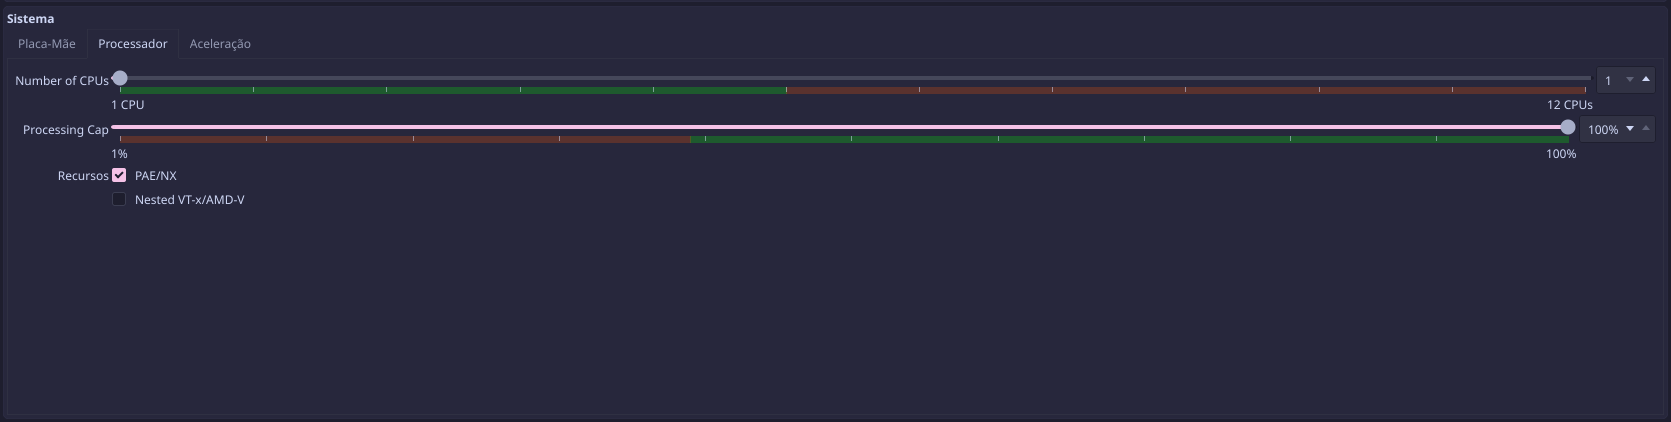
\includegraphics[width=0.9\textwidth]{assets/config1.png}
    \caption{Configuração das máquinas virtuais pt. 1}
\end{figure}

\begin{figure}[H]
    \centering
    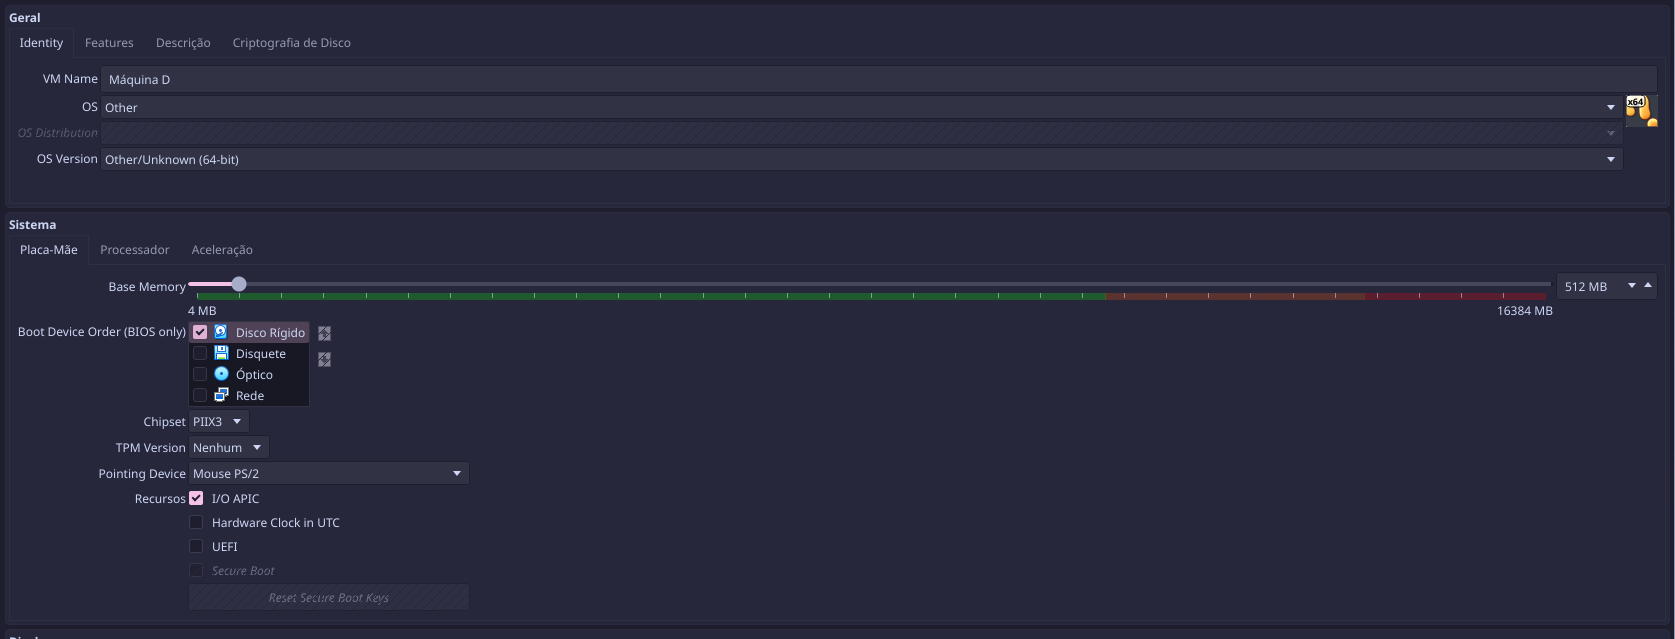
\includegraphics[width=0.9\textwidth]{assets/config2.png}
    \caption{Configuração das máquinas virtuais pt. 2}
\end{figure}

\begin{figure}[H]
    \centering
    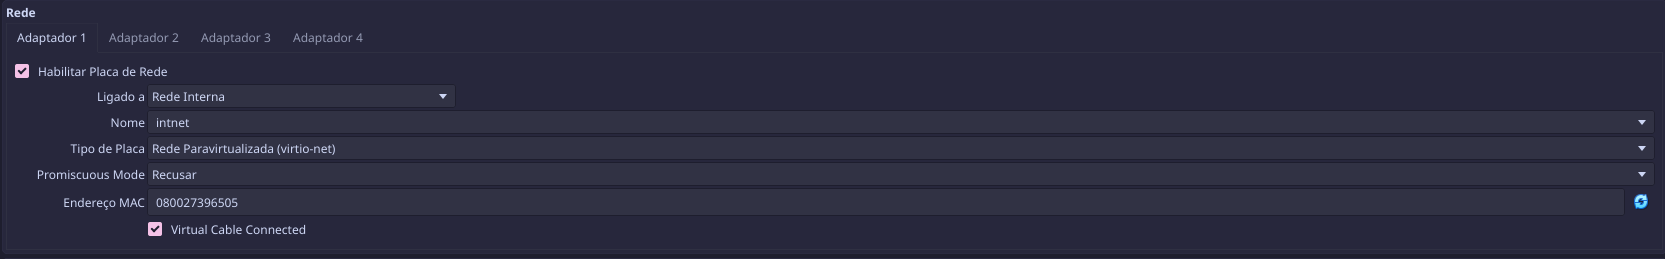
\includegraphics[width=0.9\textwidth]{assets/config3.png}
    \caption{Configuração das máquinas virtuais pt. 3}
\end{figure}

\FloatBarrier

\subsection{Conectividade entre as Máquinas}

Foram realizados testes de comunicação para validar a conectividade da rede entre as máquinas do cluster. A figura abaixo mostra o resultado das conexões de cada máquina:

\begin{figure}[H]
    \centering
    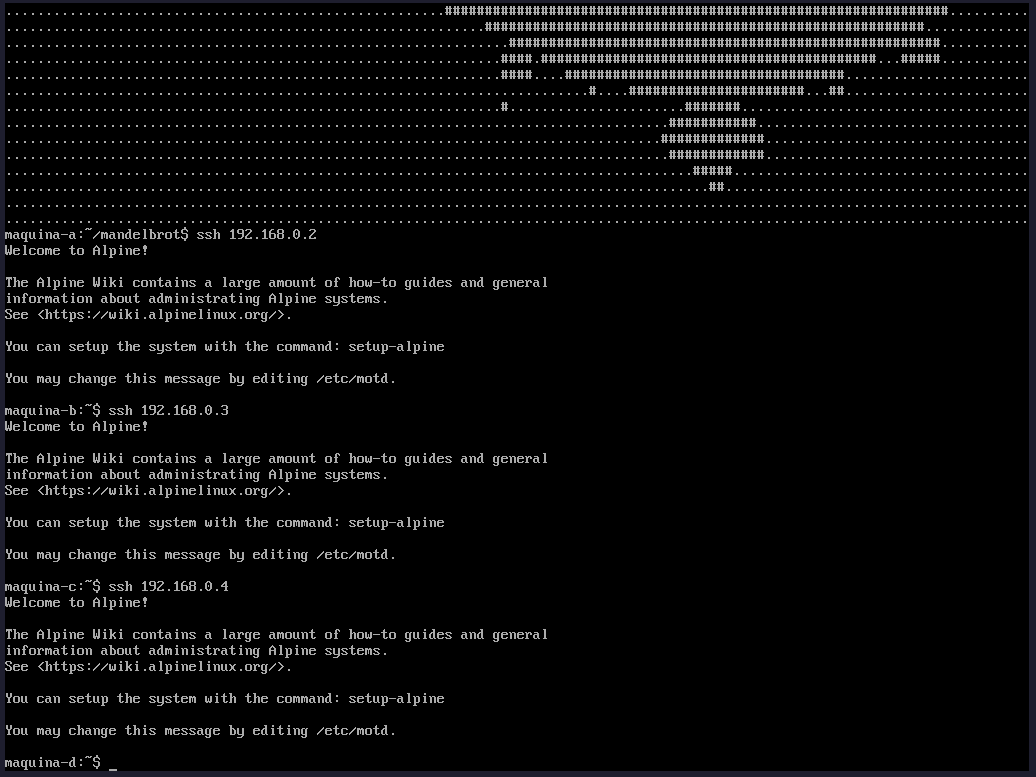
\includegraphics[width=0.8\textwidth]{assets/ssh.png}
    \caption{Teste de acesso remoto via SSH}
\end{figure}

\FloatBarrier

\chapter{Estratégia de Paralelização}

\section{Divisão de Carga}

A aplicação distribui as linhas da imagem do conjunto de Mandelbrot entre todos os processos MPI disponíveis.

Inicialmente, o processo mestre (rank 0) recebe os parâmetros de entrada:

\begin{itemize}
    \item Número de linhas;
    \item Número de colunas;
    \item Número máximo de iterações.
\end{itemize}

Esses valores são enviados para todos os processos por meio da função:

\begin{verbatim}
MPI_Bcast()
\end{verbatim}

A quantidade de linhas atribuídas a cada processo é calculada através da divisão inteira:

\begin{verbatim}
base_rows = max_row / size
\end{verbatim}

Caso a divisão não seja exata, as linhas restantes são distribuídas entre os primeiros processos.

Cada processo calcula apenas o subconjunto de linhas sob sua responsabilidade, reduzindo significativamente o tempo total de processamento.

\section{Comunicação entre Processos}

A comunicação ocorre em duas etapas principais:

\begin{enumerate}
    \item Distribuição dos parâmetros de execução utilizando
    \texttt{MPI\_Bcast}.
    
    \item Coleta dos resultados parciais utilizando
    \texttt{MPI\_Gatherv}.
\end{enumerate}

A função \texttt{MPI\_Gatherv} foi utilizada porque diferentes processos podem receber quantidades distintas de linhas quando o número total de linhas não é divisível pela quantidade de processos.

O processo mestre reúne todos os blocos calculados e monta a imagem final do fractal.

\chapter{Código-Fonte}

O código-fonte completo da aplicação é apresentado a seguir.

\small

\begin{verbatim}
#include <mpi.h>
#include <stdio.h>
#include <stdlib.h>

int main(int argc, char **argv) {
  MPI_Init(&argc, &argv);

  int rank, size;

  MPI_Comm_rank(MPI_COMM_WORLD, &rank);
  MPI_Comm_size(MPI_COMM_WORLD, &size);

  int max_row, max_column, max_n;

  if (rank == 0) {
    if (argc != 4) {
      fprintf(stderr, "Uso: %s linhas colunas iteracoes\n", argv[0]);
      MPI_Abort(MPI_COMM_WORLD, 1);
    }

    max_row = atoi(argv[1]);
    max_column = atoi(argv[2]);
    max_n = atoi(argv[3]);
  }

  MPI_Bcast(&max_row, 1, MPI_INT, 0, MPI_COMM_WORLD);
  MPI_Bcast(&max_column, 1, MPI_INT, 0, MPI_COMM_WORLD);
  MPI_Bcast(&max_n, 1, MPI_INT, 0, MPI_COMM_WORLD);

  int base_rows = max_row / size;
  int remainder = max_row % size;

  int local_rows = base_rows + (rank < remainder ? 1 : 0);

  int start_row = rank * base_rows +
                  (rank < remainder ? rank : remainder);

  char *local = malloc(local_rows * max_column);

  for (int r = 0; r < local_rows; r++) {
    int global_r = start_row + r;

    for (int c = 0; c < max_column; c++) {
      float zr = 0.0f;
      float zi = 0.0f;

      float cr =
        (float)c * 2.0f / max_column - 1.5f;

      float ci =
        (float)global_r * 2.0f / max_row - 1.0f;

      int n = 0;

      while ((zr * zr + zi * zi) < 4.0f &&
             ++n < max_n) {

        float new_zr =
          zr * zr - zi * zi + cr;

        float new_zi =
          2.0f * zr * zi + ci;

        zr = new_zr;
        zi = new_zi;
      }

      local[r * max_column + c] =
        (n == max_n) ? '#' : '.';
    }
  }

  char *global = NULL;
  int *recvcounts = NULL;
  int *displs = NULL;

  if (rank == 0) {
    global = malloc(max_row * max_column);

    recvcounts = malloc(size * sizeof(int));
    displs = malloc(size * sizeof(int));

    int offset = 0;

    for (int p = 0; p < size; p++) {
      int rows =
        base_rows + (p < remainder ? 1 : 0);

      recvcounts[p] = rows * max_column;
      displs[p] = offset;

      offset += recvcounts[p];
    }
  }

  MPI_Gatherv(
    local,
    local_rows * max_column,
    MPI_CHAR,
    global,
    recvcounts,
    displs,
    MPI_CHAR,
    0,
    MPI_COMM_WORLD
  );

  if (rank == 0) {

    for (int r = 0; r < max_row; r++) {
      for (int c = 0; c < max_column; c++) {
        putchar(global[r * max_column + c]);
      }
      putchar('\n');
    }

    free(global);
    free(recvcounts);
    free(displs);
  }

  free(local);

  MPI_Finalize();

  return 0;
}
\end{verbatim}

\normalsize

\chapter{Compilação e Execução}

\section{Compilação}

A aplicação foi compilada utilizando o compilador MPI:

\begin{verbatim}
mpicc mandelbrot.c -o mandelbrot
\end{verbatim}

\section{Execução}

O seguinte comando foi utilizado para executar a aplicação no cluster:

\begin{verbatim}
mpirun -np 1 --hostfile hosts ./build/mandelbrot 40 80 128000
\end{verbatim}

Onde:

\begin{itemize}
    \item \texttt{-np 1}: executa 1 processo MPI;
    \item \texttt{--hostfile hosts}: máquinas participantes;
    \item \texttt{40}: exemplo de número de linhas;
    \item \texttt{80}: exemplo de número de colunas;
    \item \texttt{12800}: número máximo de iterações.
\end{itemize}

\chapter{Resultados Obtidos}

A Figura abaixo apresenta a execução correta da aplicação distribuída e o resultado gerado para a entrada de teste.

\begin{figure}[H]
    \centering
    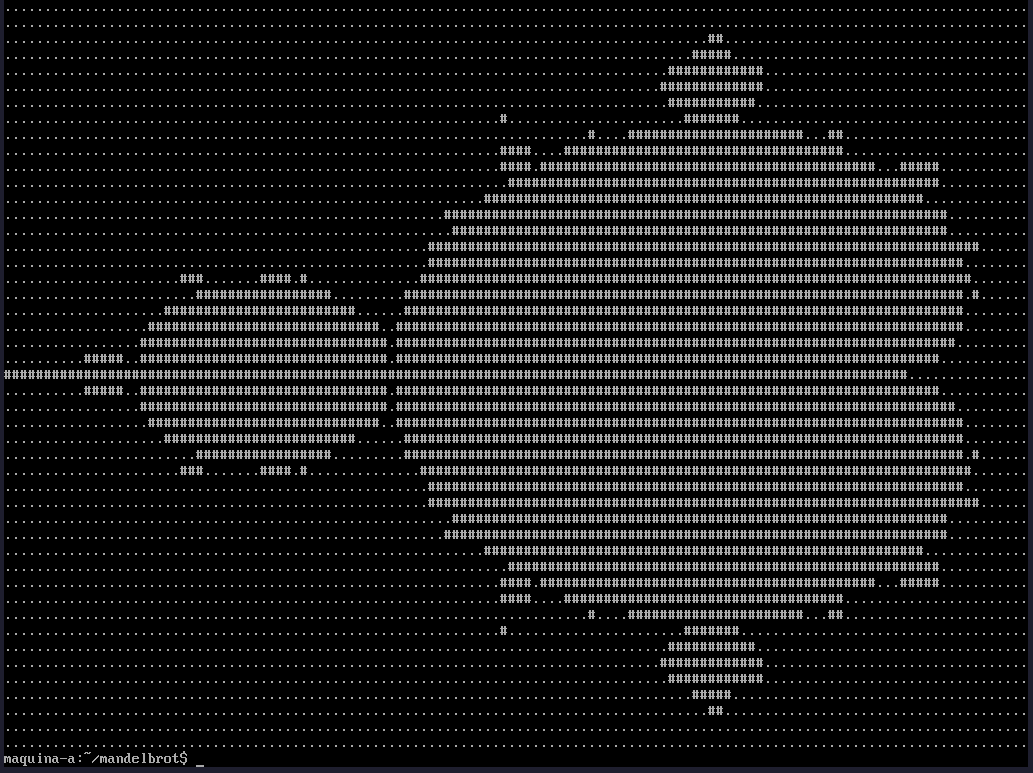
\includegraphics[width=\textwidth]{assets/resultado.png}
    \caption{Resultado da execução da aplicação MPI}
\end{figure}

\FloatBarrier

\chapter{Dificuldades Encontradas e Aprendizados}

Durante o desenvolvimento da atividade foi encontrado dificuldades relacionadas à compreensão o funcionamento das operações coletivas do MPI, especialmente a utilização da função \texttt{MPI\_Gatherv}, necessária para reunir blocos de tamanhos diferentes calculados pelos processos.

Como aprendizado, a atividade permitiu compreender conceitos fundamentais de computação paralela, incluindo:

\begin{itemize}
    \item Modelo SPMD (Single Program Multiple Data);
    \item Comunicação coletiva com MPI;
    \item Balanceamento de carga;
    \item Distribuição de tarefas entre múltiplos processos;
    \item Execução distribuída em clusters.
\end{itemize}

Além disso, foi possível observar na prática como problemas independentes, como o cálculo do conjunto de Mandelbrot, podem ser paralelizados de forma eficiente para reduzir o tempo de processamento.

\end{document}
